\documentclass[a4paper,11pt]{article}

\usepackage[english,greek]{babel}
\usepackage{graphicx}

\usepackage[utf8x]{inputenc}

\usepackage{amsfonts , amssymb , amsmath}
\usepackage{float}
\usepackage{multirow}

\usepackage{amsmath}

\title{\latintext TexProject \LaTeX\ Project}
\author{Ονοματεπώνυμο: Νικόλαος Ιλαρίδης \\ ΑΕΜ: 4524}
\date{\today}



\begin{document}
	
	\maketitle
	
	\section{Πρώτη Ασκηση}
		\begin{center}
			\emph{\greektext \begin{tiny}A\end{tiny}\begin{scriptsize}Β\end{scriptsize}\begin{footnotesize}\end{footnotesize}\begin{small}Γ\end{small}\begin{normalsize}Δ\end{normalsize}\begin{normalsize}Ε\end{normalsize}\begin{large}Ζ\end{large}\begin{Large}Η\end{Large}\begin{huge}Θ\end{huge}\begin{Huge}Ι\end{Huge}\begin{Huge}κ\end{Huge}\begin{huge}λ\end{huge}\begin{Large}μ\end{Large}\begin{large}ν\end{large}\begin{normalsize}ξ\end{normalsize}\begin{small}ο\end{small}\begin{footnotesize}π\end{footnotesize}\begin{scriptsize}ρ\end{scriptsize}\begin{tiny}σ\end{tiny}}
		\end{center}
		
\vspace{5cm}

	\section{Δεύτερη Άσκηση}
	\begin{center}
		
		\latintext {
			\emph{\begin{Huge}Normal Italics\end{Huge} \textbf{\begin{Huge}Bold\end{Huge}}}\\
			\begin{Huge}E\end{Huge}\emph{\begin{Huge}mphasized\end{Huge} \underline{\begin{Huge}Underlined\end{Huge}}}
		}
	\end{center}	
	
	\pagebreak
	
	\section{Τρίτη Άσκηση}
	\begin{center}
		$a^2 + b^2 = c^2$
		$$e^{\latintext i \pi} = -1$$
		$\pi = \dfrac{c}{d}$
		$$\frac{d}{dx}\int_{a}^{x}f(s)ds = f(x)$$
		$$f(x) = \sum_{i=0}^{\infty}\frac{f^{(i)}(0)}{i!}x^i$$
		$$\textbf{\latintext{Ax} = \latintext{b}}$$
		$$\|\mathbf{x}+\mathbf{y}\|\leq\|\mathbf{x}\|+\|\mathbf{y}\|$$
		
		
		\begin{align}
			\mathbf{I} = \begin{pmatrix}
				1 & 0 & 0 & 0 \\
				0 & 1 & 0 & 0 \\
				0 & 0 & 1 & 0 \\
				0 & 0 & 0 & 1
			\end{pmatrix}
		\end{align}
		
		
		\begin{align}
			\mathbf{I} = \begin{bmatrix}
				1 & 0 & 0 & 0 \\
				0 & 1 & 0 & 0 \\
				0 & 0 & 1 & 0 \\
				0 & 0 & 0 & 1
			\end{bmatrix}
		\end{align}
		
		
		
		\begin{align}
			\mathbf{I} = \begin{Bmatrix}
				1 & 0 & 0 & 0 \\
				0 & 1 & 0 & 0 \\
				0 & 0 & 1 & 0 \\
				0 & 0 & 0 & 1
			\end{Bmatrix}
			,\quad 
			\mathbf{I} = \begin{vmatrix}
				1 & 0 & 0 & 0 \\
				0 & 1 & 0 & 0 \\
				0 & 0 & 1 & 0 \\
				0 & 0 & 0 & 1
			\end{vmatrix}
			,\quad 
			\mathbf{I} = \begin{Vmatrix}
				1 & 0 & 0 & 0 \\
				0 & 1 & 0 & 0 \\
				0 & 0 & 1 & 0 \\
				0 & 0 & 0 & 1
			\end{Vmatrix}
		\end{align}
		
	\end{center}
	
	\pagebreak
	
	\section{Τέταρτη Άσκηση}
	\begin{center}
		\begin{tabular}{l c r}
			\greektext \emph{Τέφας} & \emph{2} & \emph{3}\\
			\greektext \emph{Πήτας} & \emph{5} & \emph{6}\\
			\greektext \emph{Λάσκαρης} & \emph{8} & \emph{9}
			
		\end{tabular}
		
		\vspace{1cm}
		
		\begin{tabular}{| l | c | r |}
			\greektext \emph{Κοτρόπουλος} & \emph{6} & \emph{3}\\
			\greektext \emph{Πήτας} & \emph{5} & \emph{6}\\
			\greektext \emph{Νικολαΐδης} & \emph{8} & \emph{9}
			
		\end{tabular}
		
		\vspace{1cm}
		
		\begin{tabular}{| l | c | r |}
			\hline
			\emph{1}&\emph{2}&\emph{3}\\ \hline
			\emph{4}&\emph{5}&\emph{6}\\ \hline
			\emph{7}&\emph{8}&\emph{9}\\ 
			\hline
		\end{tabular}
		
		\vspace{1cm}
		
		
		\begin{tabular}{| l | c | r |}
			\hline
			\emph{1}&\emph{2}&\emph{3}\\ \hline
			\emph{4}&\emph{5}&\emph{6}\\ \hline
			\emph{7}&\emph{8}&\emph{9}\\ 
			\hline
		\end{tabular}
		
		
		\vspace{1cm}
		
		\begin{tabular}{ |l|l|l| }
			\hline
			\multicolumn{3}{ |c| }{\greektext \emph{Μέλη ΔΕΠ Πληροφορικής}}\\
			\hline
			\greektext \emph{Λέκτορες} & \latintext \emph{VD} & \greektext \emph{Δραζιώτης Κωνσταντίνος}\\ 
			\hline
			\multirow{2}{*}{\greektext Επίκουροι} & \latintext \emph{LN} & \greektext \emph{Λάσκαρης Νικόλαος}\\
			& \latintext \emph{TG} & \greektext \emph{Τσουμάκας Γρηγόριος}\\
			\hline
			\multirow{3}{*}{\greektext \emph{Αναπληρωτές}} & \latintext \emph{TA} & \greektext \emph{Τέφας Αναστάσιος}\\
			& \latintext \emph{PN} & \greektext \emph{Πλέρος Νίκος}\\
			& \latintext \emph{PA} & \greektext \emph{Παπαδόπουλος Απόστολος}\\
			\hline
			\multirow{3}{*}{\emph{Καθηγητές}} & \latintext \emph{KC} & \greektext \emph{Κοτρόπουλος Κωνσταντίνος}\\
			& \latintext \emph{PI} & \greektext \emph{Πήτας Ιωάννης}\\
			& \latintext \emph{VI} & \greektext \emph{Βλαχάβας Ιωάννης}\\
			\hline	
			
		\end{tabular}
	\end{center}
	
	\pagebreak
	
	\section{Πέμπτη Άσκηση}
	\begin{flushleft}
		\begin{itemize}
			\item \greektext{\emph{Τέφας}}
			\item \greektext{\emph{Μπουζάς}}
			\item \greektext{\emph{Μπρούζα}}
			\item \greektext{\emph{Λάσκαρης}}
			\item \greektext{\emph{Κοτρόπουλος}}
			\item \greektext{\emph{Πήτας}}
			\item \greektext{\emph{Νικολαΐδης}}
		\end{itemize}
		\begin{enumerate}
			\item \greektext{\emph{Τέφας}}
			\item \greektext{\emph{Μπουζάς}}
			\item \greektext{\emph{Μπρούζα}}
			\item \greektext{\emph{Λάσκαρης}}
			\item \greektext{\emph{Κοτρόπουλος}}
			\item \greektext{\emph{Πήτας}}
			\item \greektext{\emph{Νικολαΐδης}}
		\end{enumerate}
		
		\begin{enumerate}
			\greektext{
				\item[\textbf{(α)}] \emph {Τέφας}
				\item[\textbf{(β)}] \emph {Μπουζάς}
				\item[\textbf{(γ)}] \emph{Μπρούζα}
				\item[\textbf{(δ)}] \emph{Λάσκαρης}
				\item[\textbf{(ε)}] \emph{Κοτρόπουλος}
				\item[\textbf{(ζ)}] \emph{Πήτας}
				\item[\textbf{(η)}] \emph{Νικολαΐδης}
			}
		\end{enumerate}
		
	\end{flushleft}
			
	\pagebreak
	
		\section{Έκτη Άσκηση}
	\begin{center}
		\emph{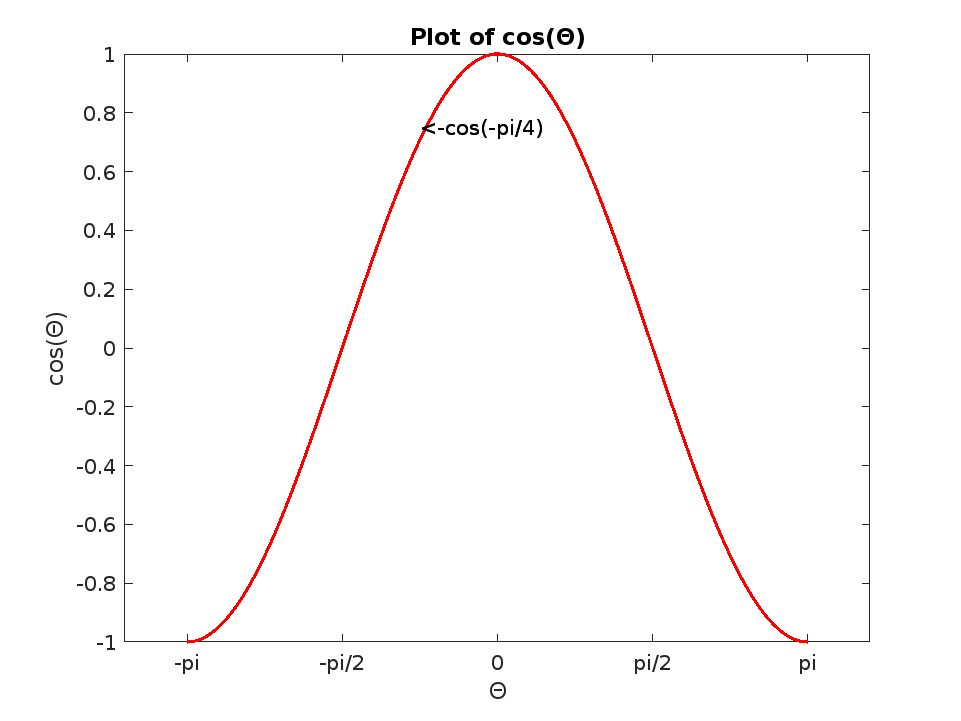
\includegraphics[scale=0.75]{cosfun.png}}
		\emph{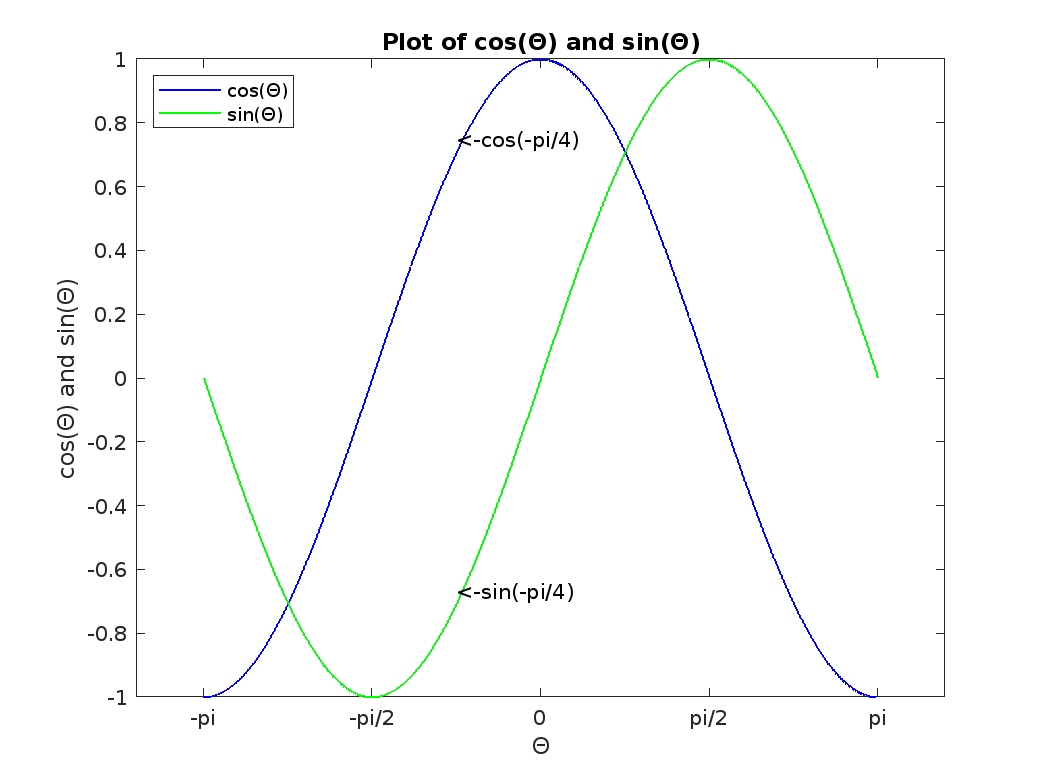
\includegraphics[scale=0.75]{cmb_fun.png}}
	\end{center}
	
	
	
\end{document}


